\documentclass{beamer}
\usepackage{../../shared/styles/custom}
\usepackage{../../shared/styles/conventions}

%\beamerdefaultoverlayspecification{<+->}
% \newcommand{\data}{\mathcal{D}}
% \newcommand\Item[1][]{%
% 	\ifx\relax#1\relax  \item \else \item[#1] \fi
% 	\abovedisplayskip=0pt\abovedisplayshortskip=0pt~\vspace*{-\baselineskip}}

\graphicspath{ {./SVM/} }

\title{SVM Soft Margin Classification}
\date{\today}
\author{Nipun Batra}
\institute{IIT Gandhinagar}
\begin{document}
	\maketitle
	
{
	\setbeamercolor{background canvas}{bg=}
	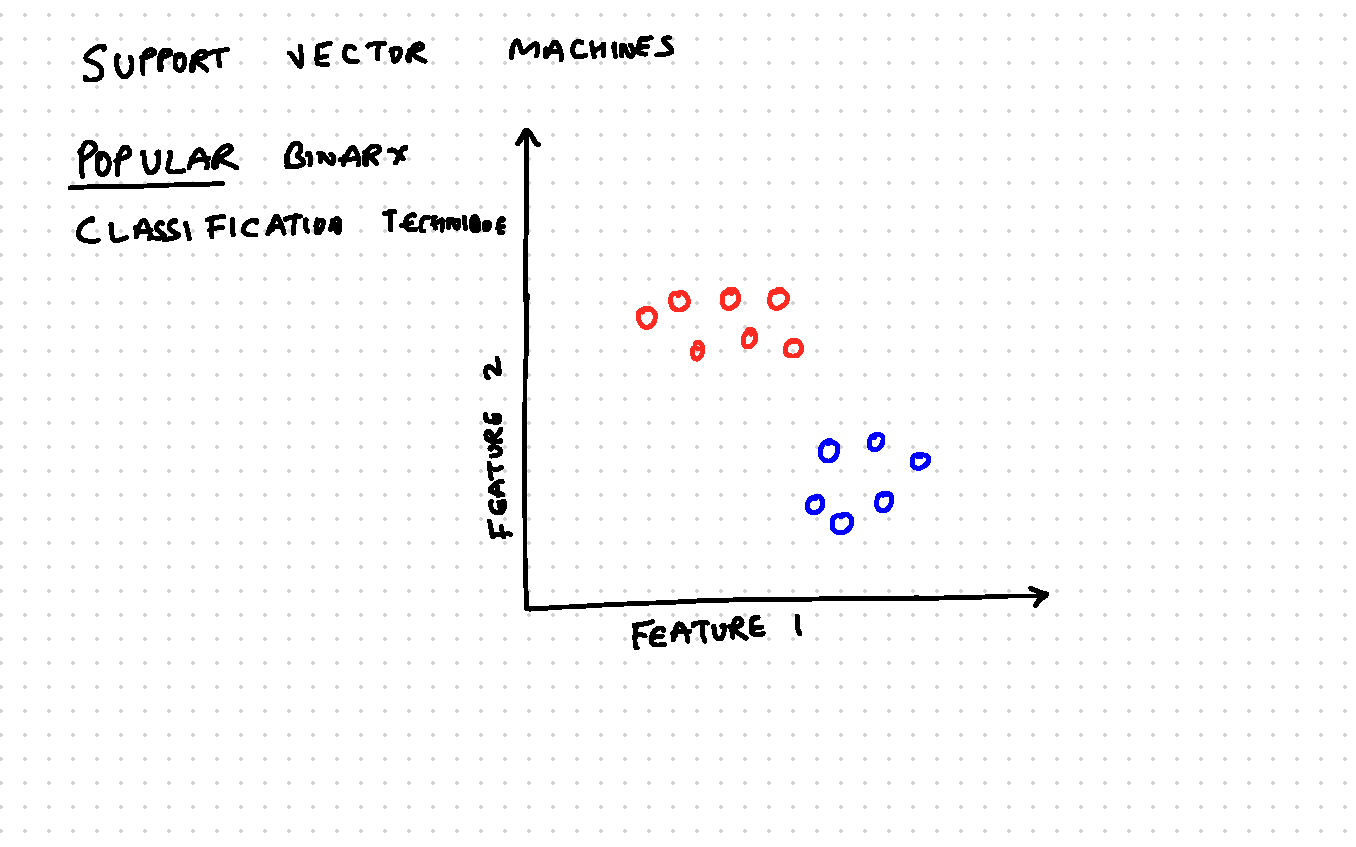
\includepdf[page=50]{../assets/Svm-notes.pdf}
}

	\begin{frame}\textbf{Answer:} b) Data has some noise and outliers - soft margin allows controlled violations.
	
\end{popquizbox}
	\end{frame}

	\begin{frame}In Dual:
		$$\minimize \sum_{i=1}^{n}\valpha_{i} - \sum_{i=1}^{n}\sum_{j=1}^{n}\valpha_{i}\valpha_{j}y_{i}y_{j}\vx_{i} \cdot \vx_{j}$$
		s.t.
		$$0 \leq \valpha_{i} \leq C \text{\hspace{0.3cm}\&\hspace{0.3cm}} \sum_{i=1}^{n}\valpha_{i}y_{i} = 0$$
		
	\end{frame}

{
	\setbeamercolor{background canvas}{bg=}
	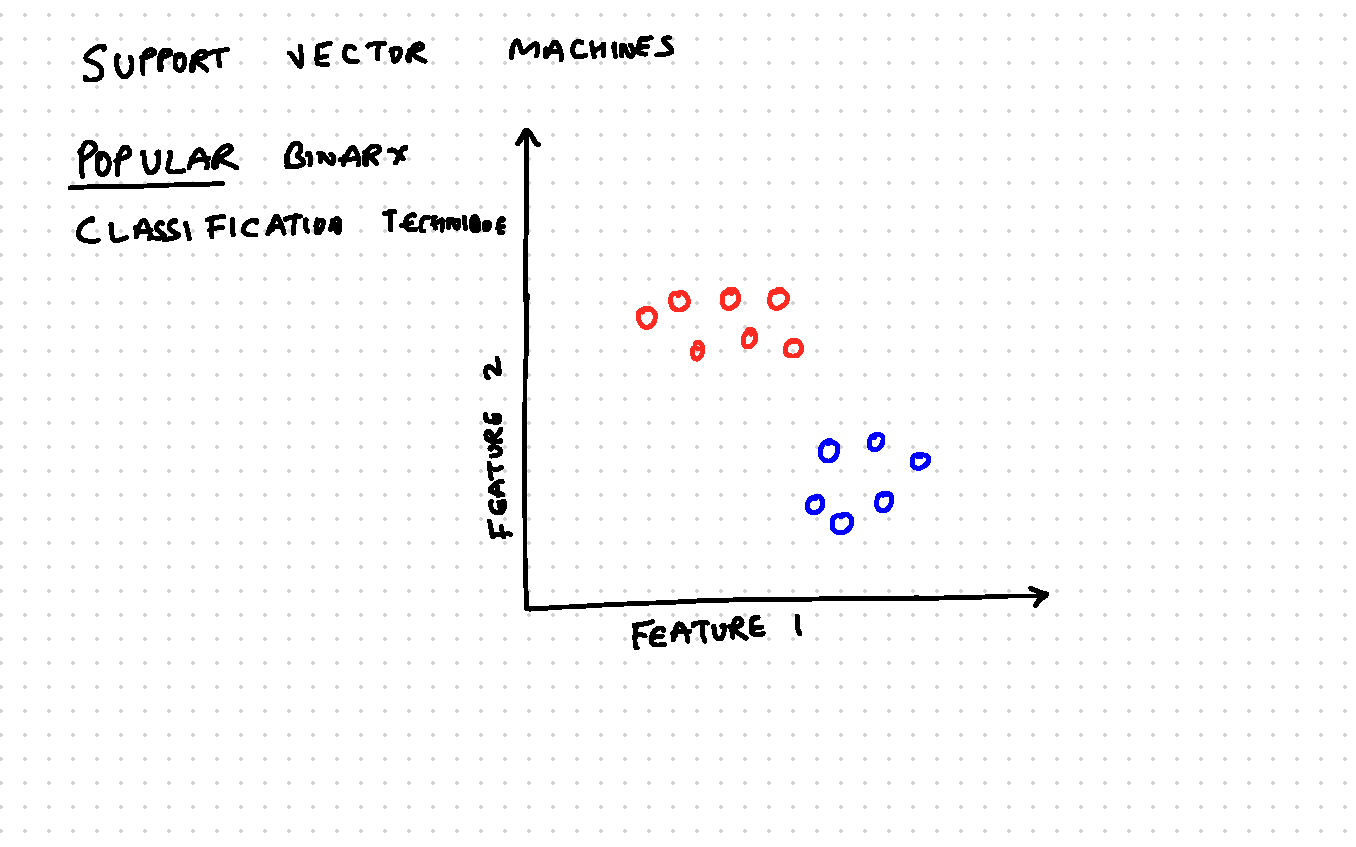
\includepdf[page=59-61]{../assets/Svm-notes.pdf}
}

\begin{frame}\textbf{Answer:} b) The model tries to classify all training points correctly - high variance!

\end{popquizbox}
\end{frame}

\begin{frame}\textbf{Answer:} b) C $\rightarrow \infty$ - No violations allowed!
	
\end{popquizbox}
	\end{frame}
	
	\begin{frame}\textbf{Answer:} c) Misclassified - since $\xi_i > 1$!
	
\end{popquizbox}
	\end{frame}

	\begin{frame}\textbf{Answer:} b) Convex but not differentiable at $y_i(\vw \cdot \vx_i + b) = 1$!
	
\end{popquizbox}
	\end{frame}

	\begin{frame}{SVM Formulation in the Loss + Penalty Form}
		$\therefore$ Objective is:
		$$\minimize C \sum \xi_{i} + \frac{1}{2}\norm{\vw}^{2}$$
		$$\implies \minimize C \sum_{i=1}^{N} \max\big[0, 1 - y_{i}(\vw \cdot \vx_{i} + b)\big] + \frac{1}{2}\norm{\vw}^{2}$$
		$$\implies \minimize \underbrace{\sum_{i=1}^{N}\max \big[0, 1-y_{i}(\vw \cdot \vx_{i} + b)\big]}_\text{Loss} + \underbrace{ \frac{1}{2C}\norm{\vw}^{2}}_\text{Regularisation}$$
	\end{frame}

{
	\setbeamercolor{background canvas}{bg=}
	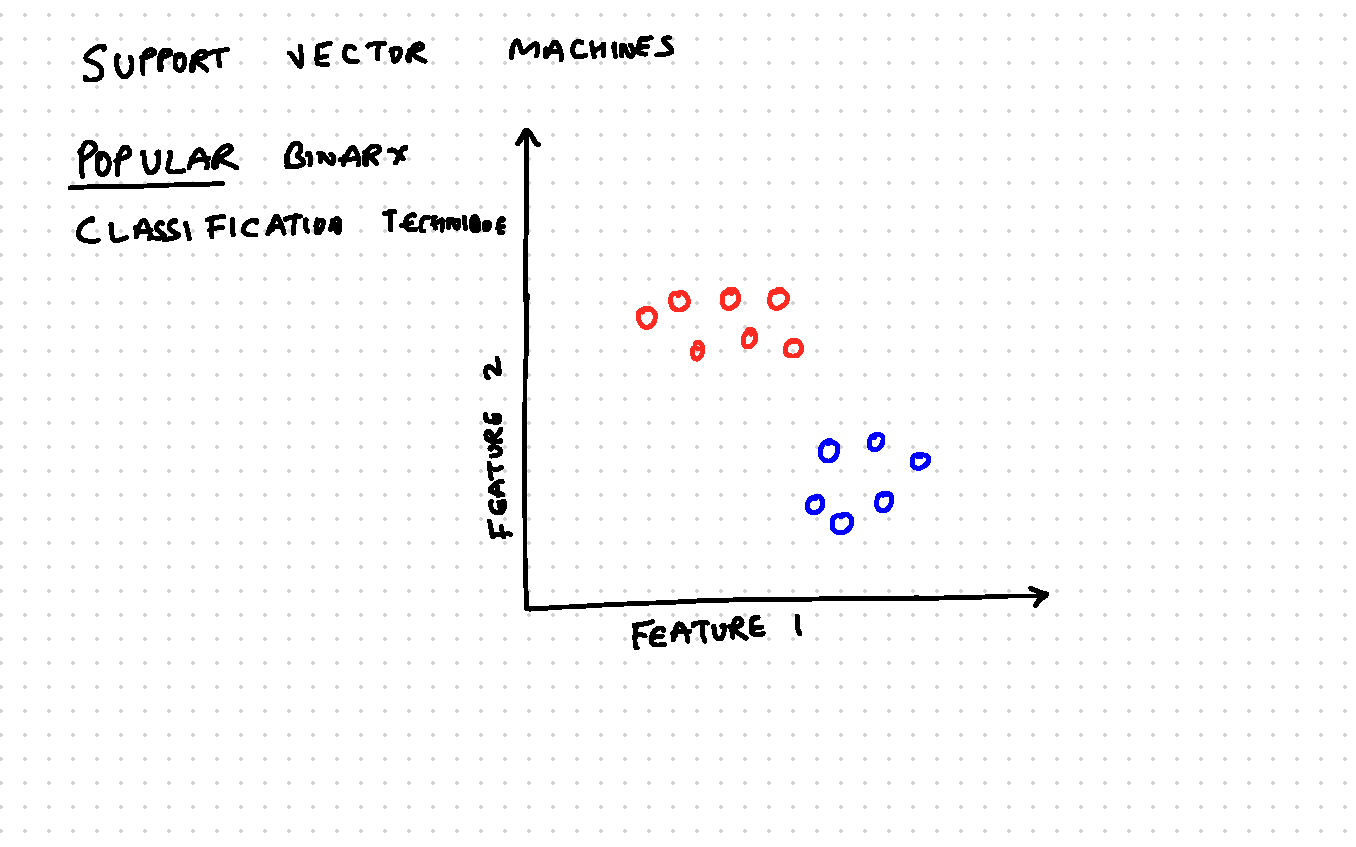
\includepdf[page=62]{../assets/Svm-notes.pdf}
}

	\begin{frame}{Loss Function for Sum (Hinge Loss)}
		Loss function is $\sum_{i=1}^{N}\max\big[0, 1 - y_{i}(\vw \cdot \vx_{i} + b)\big]$ \\
		\begin{itemize}
\item Case I 
			\hspace{0.5cm} $y_{i}(\vw \cdot \vx_{i} + b) = 1$ \\
			
			Lies on Margin: $Loss_{i}$ = 0 \\
		
			\item Case II \\
			\hspace{0.5cm} $y_{i}(\vw \cdot \vx_{i} + b) > 1$ \\
			$Loss_{i} = 0$ \\ 
			
			\pause
\item Case III \\
			\hspace{0.5cm} $y_{i}(\vw \cdot \vx_{i} + b) < 1$ \\
			$Loss_{i} \neq 0$
		\end{itemize}

	\end{frame}
	\begin{frame}{Hinge Loss Continued}
		Q) Is hinge loss convex and differentiable? \\
		\hspace{0.5cm}Convex: $\checkmark$ \\
		\hspace{0.5cm}Differentiable: X\\
		\hspace{0.5cm}Subgradient: $\checkmark$
	\end{frame}
	\begin{frame}{SVM Loss is Convex}
		
		Hinge Loss $\sum(\max[0, (1-y_{i}(\vw \cdot \vx_{i}+b))]$ is convex \\
		\vspace{1cm}
		Penalty $\frac{1}{2}\norm{\vw}^{2}$ is convex \\
		\vspace{1cm}
		$\therefore$ SVM loss is convex
	\end{frame}
	
\end{document}
